\documentclass[a4paper]{article}
\usepackage{graphicx}
\usepackage{float}
\usepackage{pgfplots}
\pgfplotsset{compat=1.18}
\usepackage{listings}
\usepackage{enumitem}
\usepackage{cancel}
\usepackage{amsmath}
\usepackage{amssymb}
\usepackage{ebproof}
\usepackage{pgfplots}
\usepackage{tikz-cd}
\usepackage{forest}
\usetikzlibrary{decorations.pathreplacing} % for angle arc
\usetikzlibrary{angles, quotes, calc} % for drawing angles
\usepackage{color}   %May be necessary if you want to color links
\usepackage{hyperref}
\hypersetup{
    colorlinks=true, %set true if you want colored links
    linktoc=all,     %set to all if you want both sections and subsections linked
    linkcolor=black,  %choose some color if you want links to stand out
}


\usepackage{mathtools}
\DeclarePairedDelimiter\ceil{\lceil}{\rceil}
\DeclarePairedDelimiter\floor{\lfloor}{\rfloor}

\usepackage{xcolor}
\usepackage{tcolorbox}

% Define a custom tcolorbox environment for examples
\newtcolorbox{examplebox}[2][]{
  colback=blue!2!white,   % Background color
  colframe=blue!30!black, % Border color
  title=#2,          % Title of the box
  boxrule=0mm,          % Thickness of the border                % Rounded corners
  fonttitle=\bfseries,    % Title font style
  width=\textwidth,  
  #1 % Width of the box (adjustable)
}

\newtcolorbox{definition} {
  colback=green!5!white,   % Background color
  colframe=green!75!black, % Border color
  title=Definizione,          % Title of the box
  boxrule=0.5mm,          % Thickness of the border                % Rounded corners
  fonttitle=\bfseries,    % Title font style
  width=\textwidth,       % Width of the box (adjustable)
}



\definecolor{codegreen}{rgb}{0,0.6,0}
\definecolor{codegray}{rgb}{0.5,0.5,0.5}
\definecolor{codepurple}{rgb}{0.58,0,0.82}
\definecolor{backcolour}{rgb}{0.95,0.95,0.92}

\lstdefinestyle{mystyle}{
    backgroundcolor=\color{backcolour},   
    commentstyle=\color{codegreen},
    keywordstyle=\color{magenta},
    numberstyle=\tiny\color{codegray},
    stringstyle=\color{codepurple},
    basicstyle=\ttfamily\footnotesize,
    breakatwhitespace=false,         
    breaklines=true,                 
    captionpos=b,                    
    keepspaces=true,                 
    numbers=left,                    
    numbersep=5pt,                  
    showspaces=false,                
    showstringspaces=false,
    showtabs=false,                  
    tabsize=2
}

\lstset{style=mystyle}

\makeatletter
\renewcommand*\env@matrix[1][*\c@MaxMatrixCols c]{%
  \hskip -\arraycolsep
  \let\@ifnextchar\new@ifnextchar
  \array{#1}}
\makeatother
\usepackage{tikz}
\usepackage{booktabs}
\title{Algoritmi}
\author{Università di Verona\\Imbriani Paolo -VR500437\\Professor Roberto Segala}

\begin{document}

\begin{figure}
    \centering
    
\includegraphics[width=0.3\textwidth]{UniversityofVerona.png}
    \label{fig:centered-image}
\end{figure}

\maketitle 

\pagebreak

\tableofcontents

\pagebreak

\section{Introduzione agli algoritmi}


Ci sono diverse definizioni di 'algoritmo' ma quella più semplice per definirlo è una sequenza di istruzioni volta a risolvere un problema. In maniera più semplice, possiamo definirlo come una ricetta. Le ricette sono delle istruzioni per creare dei piatti: queste istruzioni sono precise tuttavia possono avere anche delle varianti. Il problema non è trovare la ricetta, ma capire quale sia quella gisuta da utilizzare in base al problema posto. 
\\\\
In questo corso impararemo come \textit{decidere}. Studiare i diversi approcci e il metodo migliore per affrontare un problema.
Capiremo come confrontare gli algoritmi fra di loro.

\subsection{Complessità}

Classifichiamo gli algoritmi in base alla loro complessità ovvero quanto tempo ci mettono per essere completati. Il nostro obiettivo è quello non di misurare il tempo in sè (poiché può dipendere dal tipo di macchina che utilizziamo) che impiega un programma a finire ma piuttosto capire il numero di istruzioni elementari che vengono impiegate per risolvere il problema.
\\\\
La complessità non è un numero bensì una funzione, poiché mappa la dimensione del problema in numero di istruzioni da eseguire. Per esempio, quando si parla di dimensione di una matrice ci si viene più comodo vedere il numero di colonne e righe piuttosto che contare il numero di elementi all'interno della matrice. La dimensione del problema è un insieme di oggetti, tipicamente un insieme di numeri che ci permette di avere un idea chiara di capire quanto sia grande il problema. Se riusciamo a misurarlo bene, potremmo facilitarci la vita nel risolvere il problema. 

\subsection{Complessità dei costrutti e ordini di grandezza}

È doveroso stare attenti a cosa moltiplichiamo: se moltiplichiamo due vettori, il numero di operazioni da eseguire è esattamente $n$. Mentre se fossero orgnanizzate in matrici quadrate con lunghezza del lato $\sqrt{n}$ la sua complessità andrebbe ad aumentare a $O(n\sqrt{n})$.
Come si rappresentano le istruzioni di un programma?
Se sono in serie:
\[\begin{matrix}
  I_1 & c_1(n)\\
  I_2 & c_2(n)\\
  \vdots\\
  I_l & c_l(n)
\end{matrix}\]
Dove la complessità totale allora sarà:
\[\sum_{i=1}^l c_i(n)\]
oppure all'interno di un costrutto \textbf{if-else:}
\[\begin{matrix}
  \text{if cond} & c_{\text{cond}}(n)\\
  I_2 & c_1(n)\\
  \text{else}\\
  I_l & c_2(n)
\end{matrix}\]
In questo caso, come faccio a sapere la complessità totale di questi istruzioni? Per capirlo, studiamo il caso nel \textit{worst case scenario} ovvero nel caso peggiore. A volte vengono mostrati anche i casi migliore ma di solito si calcola il tempo peggiore. Quindi ci interessa specialmente il \textit{limite superiore} dell'algoritmo, quindi piuttosto che dire che la complessità è esattamente \textbf{uguale} questo numero, invece noi diremo che è \textbf{minore o uguale} del numero calcolato.

\[C(n) = c_{\text{cond}}(n) + max(c_1(n), c_2(n))\]
Mentre per un while loop? 
\[\begin{matrix}
    \text{while cond} & c_{cond}(n)\\
    I & c_0(n)
\end{matrix}\]
Sia $m$ limite superiore numero di iterazioni che esegue l'algoritmo. La complessità di questo algoritmo quindi sarà:
\[C(n) = c_{cond}(n) + m(c_{cond}(n) + c_0(n))\]
Proviamo ora a calcolare la molteplicazioni tra matrici.
Siano due matrici $A$ e $B$ rispettivamente con dimensione $n$ x $m$ e $m$ x $l$.
\begin{lstlisting}
For i <- 1 to n
    For j <- 1 to l
        C[i][j] <- 0
        For k <- 1 to m
            C[i][j] += A[i][j] * B[k][j]
\end{lstlisting}
Avere un risultato del tipo $5m + 1$ (riguardo il for più interno) è inutile perché non ci da informazioni realmente utili sulla complessità dell'algoritmo. 
Ad ogni modo contando tutti i for, avremo un risultato del tipo:

\[n(5ml + 4l + 2) + n + 1 = 5nml + 4nl + 3n + 1\]
Ci sono alcuni elementi in questa operazioni che non influiscono realmente sul risultato finale. Indi per cui, possiamo anche ometterlo all'interno del calcolo della complessità di un algoritmo.
In realtà ciò che ci interessa realmente nel risultato finale è:
\[5\colorbox{yellow}{\textbf{nml}}+ 4nl + 3n + 1\]
Infatti $nml$ è capace di dirci tutto sulla complessità dell'algoritmo e da cosa dipende. 
Quando si parla di ordine di grandezza si parla in realtà del comportamento asintotico della funzione calcolata.
\begin{definition}
\[f \in O(g)  \Longleftrightarrow \exists c > 0, \,\, \exists \overline{n}, \,\, \forall n \ge \overline{n} \, | \, f(n) \le cg(n)\]
\end{definition}
\begin{figure}[H]
    \centering
    \caption{$f \in O(g)$}
\begin{tikzpicture}
    \begin{axis}[
        axis lines = middle,
        xlabel = $x$,
        ylabel = {$\textcolor{blue}{f(n)}, \textcolor{red}{cg(n)}$},
        legend pos=north west,
        domain=2:8,
        samples=200,
        xmin=2, xmax=8, ymin=-5, ymax=30,
        width=12cm,
        height=8cm
    ]
        % Plot f(x) = exp(x) / 5
        \addplot[color=red, thick] {(exp(x))/5};
        
        % Plot g(x) = (30*ln(x)) / (sin(x) + 3)
        \addplot[color=blue, thick] {(30*ln(x))/(sin(deg(x)) + 3)};
        
        % Add a vertical line at the intersection point
        \addplot[mark=none, black, dashed, thick] coordinates {(4.8, 0) (4.8, 24)};
        \node at (axis cs:4.2,25) [anchor=west] {$\overline{n}$};
        
    \end{axis}
\end{tikzpicture}
\end{figure}

\begin{definition}
  \[f \in \Omega(g) \Longleftrightarrow \exists c > 0, \,\, \exists \overline{n}, \,\, \forall n \ge \overline{n} \, | \, f(n) \ge cg(n)\]  
  Che rispettivamente è l'inverso della funzione O grande.
\end{definition}

\begin{figure}[H]
    \centering
    \caption{$f \in \Omega(g)$}
\begin{tikzpicture}
    \begin{axis}[
        axis lines = middle,
        xlabel = $x$,
        ylabel = {$\textcolor{blue}{f(n)}, \textcolor{red}{cg(n)}$},
        legend pos=north west,
        domain=2:8,
        samples=200,
        xmin=2, xmax=8, ymin=-5, ymax=30,
        width=12cm,
        height=8cm
    ]
        % Plot f(x) = exp(x) / 5
        \addplot[color=blue, thick] {(exp(x))/5};
        
        % Plot g(x) = (30*ln(x)) / (sin(x) + 3)
        \addplot[color=red, thick] {(30*ln(x))/(sin(deg(x)) + 3)};
        
        % Add a vertical line at the intersection point
        \addplot[mark=none, black, dashed, thick] coordinates {(4.8, 0) (4.8, 24)};
        \node at (axis cs:4.2,25) [anchor=west] {$\overline{n}$};
        
    \end{axis}
\end{tikzpicture}
\end{figure}
\begin{definition}
  \[f \in \Theta(g) \Longleftrightarrow f \in O(g)  \, \wedge \, f \in \Omega(g)\]  
\end{definition}

\begin{figure}[H]
    \centering
    \caption{$f \in \Theta(g)$}
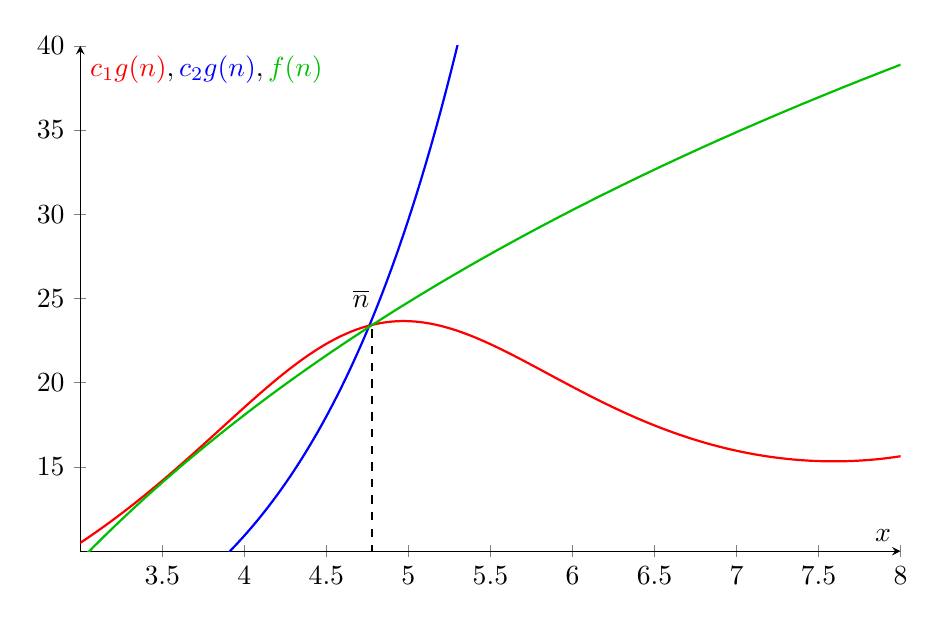
\begin{tikzpicture}
    \begin{axis}[
        axis lines = middle,
        xlabel = $x$,
        ylabel = {$\textcolor{red}{c_1g(n)}, \textcolor{blue}{c_2g(n)}, \textcolor{green!75!black}{f(n)}$},
        legend pos=north west,
        domain=2:8,
        samples=200,
        xmin=3, xmax=8, ymin=10, ymax=40,
        width=12cm,
        height=8cm
    ]
        \addplot[color=blue, thick] {(exp(x))/5};
        \addplot[color=red, thick] {(30*ln(x))/(sin(deg(x)) + 3)};
        \addplot[color=green!75!black, thick] {30*ln(x) - 23.5};

        
        % Add a vertical line at the intersection point
        \addplot[mark=none, black, dashed, thick] coordinates {(4.78, 0) (4.78, 23.65)};
        \node at (axis cs:4.6,25) [anchor=west] {$\overline{n}$};
        
    \end{axis}
\end{tikzpicture}
\end{figure}



\begin{examplebox}{Esempio 1}
Questa affermazione vale?
\[n \in O(2n)\]
Sì, perché esiste un $c$ che soddisfa $n \le c2n$.\\\\
Quest'altra affermazione vale?
\[2n \in O(n)\]
Sì perché esiste un $c$ che soddisfa $2n \le 2n$.
\end{examplebox}
\begin{examplebox}{Esempio 2}
Questa affermazione vale?
\[f \in O(g) \Longleftrightarrow g \in \Omega(g)\]
Proviamo a dimostrare. Sappiamo che esiste un $c$ e $\overline{n}$ tale che \(\forall n > \overline{n} \; f(n) \le cg(n)\). Isoliamo la g:
\[g(n) \ge \frac{1}{c} f(n)\]
Esiste quindi un c' che soddisfa la disuguaglianza. 
\[c' = \frac{1}{c}\]
\end{examplebox}
\begin{examplebox}{Esempio 3}

\[f_1 \in O(g), 
f_2 \in O(g) \Longrightarrow f_1 + f_2 \in O(g)
\]
Dobbiamo dimostrare che esiste $c_1$ e $c_2$, $\overline{n}_1$ e $\overline{n}_2$ tali che:
\[\forall n > \overline{n}_1 \; | \; f_1(n) \le c_1g(n)\]
\[\forall n > \overline{n}_2 \; | \; f_2(n) \le c_2g(n)\]
Quindi
\[\overline{n} = max(\overline{n}_1, \overline{n}_2)\]
\[f_1(n) + f_2(n) \le (c_1 + c_2)g(n)\]
    
\end{examplebox}

\begin{examplebox}{Esempio 4}
    \[f_1 \in O(g_1), f_2 \in O(g_2) \; | \; f_1f_2 \in O(g_1g_2)\]
Quindi esiste $c_1$ e $c_2$, $\overline{n}_1$ e $\overline{n}_2$ tali che:
\[\forall n > \overline{n}_1 \; | \; f_1(n) \le c_1g(n)\]
\[\forall n > \overline{n}_2 \; | \; f_2(n) \le c_2g(n)\]
\[f_1(n)f_2(n) \le c_1g_1(n)c_2g_2(n)\]
\[f_1(n)f_2(n) \le c_1c_2g_1(n)g_2(n)\]
Quindi:
 \[c = c_1c_2\] \[\overline{n} = max(\overline{n}_1, \overline{n}_2)\]
\end{examplebox}

\subsection{Ordini di grandezza per le funzioni}

L'algoritmo di ricerca $A$ termina entro n. Immaginiamo che l'algoritmo A sia il seguente:
\begin{lstlisting}
For i <- 0 to length(a) - 1
    if a[i] = x
        ret i
ret -1
\end{lstlisting}
Capiamo che la sua complessità è uguale a:
\[A \in O(n)\]
Per appurarci che la stima di complessità sia accurata dobbiamo controllare che $A \in \Omega(g)$ vuol dire che esiste uno schema di input tale per cui se $g(n)$ è il numero di passi necessari per risolvere l'istanza $n$, allora $g \in \Omega(f)$. Se riusciamo a fare questo allora $g \in \Theta(f)$ e quindi possiamo dire che la stima è accurata.
\\\\
$P \in O(f)$ vuol dire che il problema $P$ riesco a risolvere in tempo $f$. Supponiamo per assurdo che esista un algoritmo riesca a capire se l'elemento si trova nell'array o no. Possiamo capire velocemente che per contraddizione, essendo che esiste almeno un elemento dove l'algoritmo non ha guardato, siamo certi del malfunzionamento dell'algoritmo e quindi non è vero che esiste una stima di complessità più bassa di $f$.


Ora andiamo ad affrontare i tipi di algoritmi che si definiscono di "ordinamento". 
\begin{definition}
\textbf{Input}: Sequenza $(a_1, ..., a_n)$ di oggetti su cui è definita una relazione di ordinamento (in questo caso ordinamento per confronti).
\\\\
\textbf{Output}: Permutazione $(a_1', ..., a_n')$ di $(a_1, ..., a_n)$ t.c. $\forall \, i > j, \; \; a_i' \le a_j'$.
\end{definition}
Andiamo ora a vedere i diversi tipi di algoritmi di ordinamento.

\subsection{insertion$\_$sort (A)}

In questo caso la $j$ sarà chiamata variabile "invariante" ovvero che mantiene una proprietà che continua a valere nel run-time dell'algoritmo. In questo caso, la $j$ è invariante perchè tutti gli oggetti "a sinistra" di essa saranno considerati già ordinati. (Parte da 2 perché abbiamo deciso che la posizione all'interno dell'array parte da 1).

\begin{lstlisting}
for j <- 2 to length[A]
    key <- A[j]
    i <- j - 1
    while i > 0 and A[i] > key
        A[i+1] <- A[i]
        i--
    a[i+1] <- key
\end{lstlisting}
Ora dobbiamo capire quale sia la complessità di questo algoritmo. Se le cose vanno bene, l'algoritmo potrebbe terminare in $O(n)$. Tuttavia, seppur giusto, non è preciso. Infatti, nel peggiore dei casi, l'algoritmo termina in $O(n^2)$. Infatti il caso peggiore di input che mi può arrivare è un array ordinato al contrario con complessità uguale a:
\[1 + 2 + 3 + ... + n = \frac{n(n+1)}{2} \in \Theta(n^2)\]
\textit{Questo algoritmo, quanto spazio di memoria usa in più rispetto allo spazio occupato dai dati? }
\\\\
Lo spazio di memoria di questo algoritmo rimane costante a prescindere dalla dimensione del problema. Un algoritmo del genere si dice che \textit{\textbf{ordina in loco}} se la quantità di memoria extra è costante. Si parla di \textit{\textbf{stabilità}} di un algoritmo di ordinamento quando l'ordine relativo di elementi uguali non viene scambiato dall'algoritmo. Quindi:
\[\text{Se } a_i = a_j \, i < j, \text{mantiene l'ordinamento}\]


\section{Concetto di "Divide et impera"}

\subsection{Fattoriale e funzioni ricorsive}

\begin{lstlisting}
Fatt(n) 
    if n = 0
        ret 1
    else
        ret n * fatt(n - 1)
\end{lstlisting}

L'argomento della funzione ci fa capire la complessità dell'algoritmo:
\[
  T(n) = \begin{cases}
    1 & \text{se } n = 0 \\
    T(n - 1) + 1 & \text{se } n > 0
  \end{cases}
\] 
Con problemi ricorsivi si avrà una complessità con funzioni definite ricorsivamente.
Questo si risolve induttivamente:
\[
  \begin{aligned}
    T(n) & = 1 + T(n-1)\\
         & = 1 + 1 + T(n-2)\\
         & = 1 + 1 + 1 + T(n-3)\\
         & = \underbrace{1 + 1 + \ldots + 1}_{i} + T(n-i)\\
  \end{aligned}
\] 
La condizione di uscita è: \( n-i = 0 \quad n = i \) 
\[
\begin{aligned}
         & = \underbrace{1 + 1 + \ldots + 1}_{n} + T(n-n)\\
         & = n + 1 = \Theta(n)
\end{aligned}
\] 
Questo si chiama passaggio iterativo.

\begin{examplebox}{Esempio 1}
  \[
    T(n) = 2T\left(\floor*{\frac{n}{2}}\right) + n
  \] 
  Questa funzione si può riscrivere come:
  \[
  T(n) = \begin{cases}
    \text{Costante} & \text{se } n < a \\
    2T\left(\floor*{\frac{n}{2}}\right) + n & \text{se } n \ge a
  \end{cases}
  \] 

  \vspace{1em}
  \noindent
  Se la complessità fosse già data bisognerebbe soltanto verificare se è corretta.
  Usando il metodo di sostituzione:
  \[
    T(n) = cn \log n
  \] 
  sostituiamo nella funzione di partenza:
  \[
    \begin{aligned}
      T(n)  & = 2T\left(\floor*{\frac{n}{2}}\right) + n\\
            & \le 2c\left(\floor*{\frac{n}{2}}\right) \log \floor*{\frac{n}{2}} + n\\
            & \le \cancel{2} c \frac{n}{\cancel{2}} \log \frac{n}{2} + n\\
            & = cn \log n - cn \log 2 + n\\
            & \stackrel{?}{\le} cn \log n \quad \text{se } n- cn \log 2 \le 0\\
    \end{aligned}
  \] 
  \[
    c \ge \frac{n}{n \log 2} = \frac{1}{\log 2}
  \] 
  Il metodo di sostituzione dice che quando si arriva ad avere una disequazione
  corrispondente all'ipotesi, allora la soluzione è corretta se soddisfa una certa ipotesi.
\end{examplebox}

\begin{examplebox}{Esempio 2}
  \[
    T(n) = T\left(\floor*{\frac{n}{2}}\right) + T\left(\ceil*{\frac{n}{2}}\right) + 1 \quad \in O(n)
  \] 
  \[
  T(n) \le cn
  \] 
  \[
  \begin{aligned}
    T(n) & = T\left(\floor*{\frac{n}{2}}\right) + T\left(\ceil*{\frac{n}{2}}\right) + 1\\
         & \le c\left(\floor*{\frac{n}{2}}\right) + c\left(\ceil*{\frac{n}{2}}\right) + 1\\
         & = c \left( \left\lfloor \frac{n}{2} \right\rfloor + \left\lceil \frac{n}{2} \right\rceil  \right) + 1\\
         & = cn + 1 \stackrel{?}{\le} cn
  \end{aligned}
  \] 
  Il metodo utilizzato non funziona perchè rimane l'1 e non si può togliere in alcun modo.
  Per risolvere questo problema bisogna risolverne uno più forte:
  \[
  T(n) \le cn - b
  \] 
  \[
  \begin{aligned}
    T(n) & = T\left(\floor*{\frac{n}{2}}\right) + T\left(\ceil*{\frac{n}{2}}\right) + 1\\
         & \le c\left(\floor*{\frac{n}{2}}\right) -b + c\left(\ceil*{\frac{n}{2}}\right) -b + 1\\
         & = c \left( \left\lfloor \frac{n}{2} \right\rfloor + \left\lceil \frac{n}{2} \right\rceil  \right) - 2b + 1\\
         & = cn - 2b + 1 \stackrel{?}{\le} cn - b\\
         & = \underbrace{cn - b} + \underbrace{1 - b}_{\le 0} \le cn - b \quad \text{se } b \ge 1\\
  \end{aligned}
  \] 
  Se la proprietà vale per questo problema allora vale anche per il problema iniziale
  perchè è meno forte.
\end{examplebox}

\begin{examplebox}{Esempio 3}
  \[
    \begin{aligned}
      T(n) & = 3T \left( \left\lfloor \frac{n}{4} \right\rfloor \right) + n\\
           & = n + 3T \left( \left\lfloor \frac{n}{4} \right\rfloor \right)\\
           & = n + 3 \left( \left\lfloor \frac{n}{4} \right\rfloor + 3T 
           \left( \left\lfloor \frac{\left\lfloor \frac{n}{4} \right\rfloor}{4} \right\rfloor
           \right)  \right)\\
           & = n + 3 \left\lfloor \frac{n}{4} \right\rfloor + 3^2 T 
           \left( \left\lfloor \frac{n}{4^2} \right\rfloor \right)\\
           & \le n + 3 \left\lfloor \frac{n}{4} \right\rfloor + 3^2 
           \left( \left\lfloor \frac{n}{4^2} \right\rfloor + 3T \left( 
           \left\lfloor \frac{\left\lfloor \frac{n}{4^2} \right\rfloor}{4} \right\rfloor
           \right)  \right) \\
           & = n + 3 \left\lfloor \frac{n}{4} \right\rfloor + 3^2
           \left\lfloor \frac{n}{4^2} \right\rfloor + 3^3 T
           \left( \left\lfloor \frac{n}{4^3} \right\rfloor \right) \\
           & = n + 3 \left\lfloor \frac{n}{4} \right\rfloor + \ldots + 3^{i-1}
           \left\lfloor \frac{n}{4^{i-1}} \right\rfloor + 3^i T
           \left( \left\lfloor \frac{n}{4^i} \right\rfloor \right) 
    \end{aligned}
  \]


  Per trovare il caso base poniamo l'argomento di T molto piccolo:
  \[
    \begin{aligned}
      \frac{n}{4^i} & < 1\\
      4^i & > n\\
      i & > \log_4 n
    \end{aligned}
  \] 
  L'equazione diventa:
  \[
    \begin{aligned}
      & \le n + 3 \left\lfloor \frac{n}{4} \right\rfloor + \ldots + 3^{\log_4 n - 1}
      \left\lfloor \frac{n}{4^{\log_4 n - 1}} \right\rfloor + 3^{\log_4 n} c\\
    \end{aligned}
  \] 


  Si può togliere l'approssimazione per difetto per ottenere un maggiorante:
  \[
  \begin{aligned}
    & \le n \left( 1 + \frac{3}{4} + \left( \frac{3}{4} \right)^2 + \ldots +
    \left( \frac{3}{4} \right)^{\log_4 n-1} \right) + 3^{\log_4 n} c\\
    & \le n \left( \sum_{i=0}^{\infty} \left( \frac{3}{4} \right)^i \right) + c 3^{\log_4 n}\\
  \end{aligned}
  \] 
    \end{examplebox}
\begin{examplebox}{}
  Per capire l'ordine di grandezza di \( 3^{\log_4 n} \) si può scrivere come:
  \[
    3^{\log_4 n} = n^{\left( \log_n 3^{\log_4 n} \right) } = n^{\log_4 n \cdot \log_n 3}
    = n^{\log_4 3}
  \] 
  Quindi la complessità è:
  \[
  \begin{aligned}
    & = O(n) + O(n^{\log_4 3})\\
  \end{aligned}
  \] 
  Si ha che una funzione è uguale al termine noto della funzione originale e l'altra
  che è uguale al logaritmo dei termini noti. Se usassimo delle variabili uscirebbe:
  \[
    \begin{aligned}
      T(n) & = a T \left( \left\lfloor \frac{n}{b} \right\rfloor \right) + f(n)\\
           & = O(f(n)) + O(n^{\log_b a})
    \end{aligned}
  \] 
\end{examplebox}



\subsection{Master Theorem o Teorema dell'esperto}

Data una relazione di occorrenza di questa forma:

\[T(n) = a T \left( \left\lfloor \frac{n}{b} \right\rfloor \right) + f(n)\]

Distinguiamo tre casi:

\begin{enumerate}
    \item \[f(n) \in O(n^{\log_ba - \epsilon}) \Longrightarrow T(n) \in \Theta(n^{\log_ba})\]
    \item \[f(n) \in \Theta(n^{\log_ba}) \Longrightarrow T(n) \in \Theta(f(n)\log n)\]
    \item \[f(n) \in \Omega(n^{\log_ba} + \epsilon) \Longrightarrow T(n) \in \Theta(f(n))\]
\end{enumerate}

\begin{examplebox}{Esempio 1}
    \[T(n) = 9T\left(\frac{n}{3}\right) + n\]
    \[a = 3, b = 3, f(n) = n\]
    Basta che trovo un $\epsilon$ che mi dia $n$.
    \[n^{\log_b a} = n^{\log_3 9} = n^2 * n^{-\frac{1}{2}}\]
    In questo caso $\epsilon = n^{-\frac{1}{2}}$ e ci troviamo nel \textbf{PRIMO CASO} e la soluzione è $T(n) \in \Theta(n^2)$.
\end{examplebox}

\begin{examplebox}{Esempio 2}
       \[T(n) = T\left(\frac{2n}{3}\right) + 1\]
    \[a = 1, b = \frac{3}{2}, f(n) = n^0\]
    \[n^{\log_b a} = n^{\log_{\frac{3}{2}} 1} = n^0\]
    Ci troviamo nel \textbf{SECONDO CASO} e la soluzione è $T(n) \in \Theta(\log n))$
\end{examplebox}

\begin{examplebox}{Esempio 3}
    \[T(n) = 3T\left(\frac{n}{4}\right) + n \log n\]
       \[a = 3, b = 4, f(n) = n \log n\]
       Ci troviamo nel \textbf{TERZO CASO} quindi basta qualsiasi valore di $\epsilon$ basta che sia contenuto tra $\log_3 4 \le \epsilon \le 1$. La soluzione è $T(n) \in \Theta(n\log n)$.
\end{examplebox}

\begin{examplebox}{Esempio 4} 
    \[T(n) = 2T\left(\frac{n}{2}\right) + n \log n\]
       \[a = 2, b = 2, f(n) = n \log n\]
    \[n\log n \in \Omega(n^{1 + \stackrel{?}{\epsilon}}) \]
    \[\log n \in \Omega(n^\epsilon) \text{ NON VALE}\]
    Poiché un logaritmo è sempre più piccolo di un polinomio.
    Questo è un caso dove il teorema \textit{non} si applica
\end{examplebox}


\subsection{Merge Sort (A, n)}

Questo algoritmo di ordinamento \textit{ricorsivo} utilizza il concetto di \textit{divide et impera}. 

Concettualmente, un merge sort funziona come segue:

\begin{enumerate}
    \item \textbf{Dividi} l'array non ordinato in n sottoarray, ognuno contenente un elemento (un array di un elemento è considerato ordinato).
    \item \textbf{Unisci} ripetutamente i sottoarray per produrre nuovi sottoarray ordinati finché non ne rimane solo uno. Questo sarà l'array ordinato.
\end{enumerate}
La sua complessità considerando il merge con complessità lineare risulta:
\[T(n) = 2T\left(\frac{n}{2}\right) + n\]
Utilizzando il \textbf{Master Theorem} e cadendo del \textit{secondo caso} possiamo confermare che il risultato è:
\[= \Theta(n \log n)\]

\begin{lstlisting}[language=Scala]
// A e' l'array mentre p ed r sono rispettivamente l'indice di partenza e di arrivo 
mergeSort(A, p, r) // O(n log n)
    if (p < r) 
        q <- floor((p+r)/2)
        mergeSort(A, p, q)
        mergeSort(A, q+1, r)
        merge(A, p, q, r)
\end{lstlisting}
\begin{lstlisting}[language=Scala]
merge(A, p, q, r)
    i <- 1
    j <- p
    k <- q+1
    // Ordina gli elementi di A in B
    // O il lato sinistro ha finito 
    while(j <= q or k <= r) // O(n)
        if j <= q and (k > r or A[j] <= A[k])
            B[i] <- A[j]  
            j++
        else
            B[i] <- A[k] 
            k++
        i++
    // Copia gli elementi di B in A
    for i <- 1 to r-p+1  // O(n)
        A[p+i-1] <- B[i]
\end{lstlisting}
L'algoritmo è \textbf{stabile} poiché non vengono scambiati gli elementi uguali. Tuttavia non ordina \textbf{in loco} poiché utilizza uno spazio di memoria aggiuntivo.
\subsection{Heap}
L'Heap è un albero semicompleto (ogni nodo ha 2 figli ad ogni livello tranne l'ultimo  che è completo solo fino ad un certo unto) in cui i nodi contengono oggetti con relazione di ordinamento.\\\\
\textbf{\textit{Proprietà Heap:}}

\[\forall \text{ nodo, il contenuto è } \ge \text{ del contenuto dei figli}\]

\begin{figure}[H]
    \centering
    
    \begin{forest}
for tree={
    draw, % Disegna i nodi
    circle, % Forma dei nodi
    minimum size=1.5em, % Dimensione minima dei nodi
    inner sep=1pt, % Spaziatura interna dei nodi
    s sep=1.5cm % Spaziatura verticale tra i livelli
}
  [16, edge label={node[right, xshift=7pt] {1}}
    [14, edge label={node[above, yshift=7pt] {2}}
      [8, edge label={node[above, yshift=7pt] {4}}
        [1, edge label={node[above, yshift=7pt] {8}}]
        [2, edge label={node[above, yshift=7pt] {9}}]
      ]
      [9, edge label={node[above, yshift=7pt] {5}}
        [3, edge label={node[right, xshift=7pt] {10}}]
      ]
    ]
    [10, edge label={node[above, yshift=7pt] {3}}
      [2, edge label={node[above, yshift=7pt] {6}}]
      [3, edge label={node[above, yshift=7pt] {7}}]
    ]
  ]
\end{forest}    
    \label{fig:enter-label}
\end{figure}
La complessità dell'algoritmo è in base al numero di livelli dell'albero.\\\\
$\longrightarrow$ albero con $n$ livelli: 
\[\# \text{Nodi} = 2^0 + 2^1 + 2^2 + ... + 2^{n - 1} = \frac{1 - 2^n}{1-2} = 2^n - 1\]
$\longrightarrow$ albero con $n$ nodi: 
\[\# \text{Livelli} = \log_2n\]
\[\#\text{Foglie} = \frac{n}{2}\]
Le foglie di un albero sono la metà dei nodi dell'albero.

\begin{lstlisting}[language=Scala]
extractMax(H) // O(log n)
    h[1] <- H[H.heap_size()]
    H.heap_size()--
    heapify(H, 1)
\end{lstlisting}

\begin{lstlisting}[language=Scala]
heapify(H, 1) // O(log n)
    l <- left[i] // 
    r <- right[i] 
    if(l < h.heap_size() AND H[l] > H[i]
        largest <- l
    else
        largest <- i
    if m <= h.heap_size() and H[r] > H[largest]
        largest <- r
    if largest != i
        swap(H[i], H[largest])
        heapify(H, largest)
\end{lstlisting}
Creare uno heap da un array:
\begin{lstlisting}[language=Scala]
buildHeap(A) 
    A.heap_size() <- length[A]
        for i <- length[A]/2 down to 1
            heapify(A, i)
\end{lstlisting}
Immagino tutte le foglie come heap con un solo nodo. L'indice del primo nodo che non è heap corrisponde a $\frac{length(A)}{2}$ su questo allora chiamo \texttt{heapify}.

\pagebreak

\subsection{Heapsort}
\begin{lstlisting}[language=Scala]
HeapSort(A) // O(n log n)
    buildHeap(A)
    for i <- length(A) to 1
        scambia(A[1], A[i])
        heapsize(A)--
        heapify(a, i)
\end{lstlisting}
L'Heap Sort è un algoritmo che lavora \textbf{in loco} tuttavia non è \textbf{stabile}. Tuttavia riusciamo a fare una stima migliore e più corretta? 
\[n \log i = \sum_{i=1}^n \log i = \log \prod_{i=1}^n i = \log n! = \Theta(\log n^n) = \Theta(n \log n)\]
In questo caso, essere accurati non aiuta, ma abbiamo avuto la certezza che non esiste una stima migliore.
\subsection{Quicksort}
Come funziona l'algoritmo?
\begin{enumerate}
    \item Dividi prima l'array in due parti. (Partizione)
    \item  Devi essere sicuro che tutti gli elementi di sinistra siano $\le$ di quelli di destra. Ricorsivamente ordina la parte sinistra e la parte destra.
    \item A questo punto l'array è ordinato.
\end{enumerate}

\begin{lstlisting}[language=Scala]
quickSort(A, p, r)
    if (p < r) 
        q <- partition(a, p, r)
        quickSort(A, p, q)
        quickSort(A, q+1, r)
\end{lstlisting}

\begin{lstlisting}[language=Scala]
partition(A, p, r) // O(n)
    x <- A[p] // Elemento Perno
    i <- p-1
    k <- r+1
    while true
        repeat j-- until a[j] <= x        
        repeat i++ until a[i] >= x
        if i < j
            scambia(a[i], a[j])
        else
            ret j
\end{lstlisting}
Scegliamo un elemento a caso in base a quello comparato rispetto all'elemento perno tale che:
\[sx \le perno \le dx\]
Questo algoritmo non è \textbf{stabile} ma lavora \textbf{in loco}.
La sua complessità?
\[T(n) = T(\text{partition}) + T(q) + T(n-q)\]
Se il quicksort è perfettamente diviso in due, allora la sua complessità è $O(n \log n)$.
Se invece l'array è già ordinato la sua equazione di ricorrenza sarà:
\[= n + T(1) + T(n-1) = \colorbox{yellow!50!white}{$\Theta(n^2)$}\]
Tuttavia non ci aspettiamo che questo caso sia frequente e quindin nella stra grande maggioranza dei casi allora:
\[T(n) = n + T(cn) + T((1-c)n)\]
Un equazione di questo tipo sappiamo che ha come complessità $\Theta(n \log n)$.
\begin{lstlisting}[language=Scala]
rand_Partition(A, p, r)
    i <- rand(p .. r) // Ora l'elemento perno e' un elemento a caso
    scambio(A[p], A[i]
    ret partition(A, p, r)
\end{lstlisting}

\begin{align*}
    T(n) &= n + \frac{1}{n}(T(1) + T(n-1) + \frac{1}{n}(T(2) + (T-2)) + \; \dots \; + \\ 
    & \frac{1}{n}(T(n-2) + T(2)) + \frac{1}{n}(T(n-1) + T(1) = \\
    &= n + \frac{1}{n} \sum_{i}(T(i) + T(n-i))\\
    &= n + \frac{2}{n} \sum_{i} T(i) \in \colorbox{green!30!white}{$O(n \log n$)}
\end{align*}
Qualsiasi algoritmo che\textit{ lavora per confronti }deve fare almeno $O(n \log n)$. 

\section{Algoritmi di ordinamento in tempo lineare}

\subsection{Algoritmi non basati su confronti}

\subsubsection{Counting Sort}
Tuttavia possiamo trovare algoritmi che come tempo 
di esecuzione hanno tempo lineare. Come? 
Non lavorando a \textbf{confronti}. 
\\\\
Come ordinare $n$ numeri con valori da 1 a $k$?
\begin{lstlisting}[language=Scala]
countingSort(A, k)
    for i <- 1 to k 
        C[i] <- 0
    for j <- 1 to len(A)
        C[A[j]]++
    for i <- 2 to k
        C[i] <- C[i-1]+C[i]
    for j <- len(A) down to 1
        B[C[A[j]]] <- a[j]
        C[A[J]]--
\end{lstlisting}
La complessità di questo algoritmo è $O(n + k)$ dove $n$ è la lunghezza dell'array e $k$ e il range di valori.

\subsubsection{Radix Sort}

Il radix sort è un algoritmo di ordinamento che ordina gli elementi 
confrontando i singoli bit. Quello che fa è ordinare per la cifra meno
significativa, poi per la seconda cifra meno significativa e così via.


\begin{lstlisting}[language=Scala]
radixSort(A, d) // O(d(n+k))
  for i <- 1 to d
      countingSort(A, n)
\end{lstlisting}
La complessità di questo algoritmo è \[\Theta(d(n+k))\]dove $d$ è il numero di cifre e $k$ è il range di valori.
Se si vuole invece ordinare $n$ valori da 1 a $n^2 - 1$, le costanti nascoste all'interno
del $\Theta$ sono molto alte e quindi non è un algoritmo efficiente. Tuttavia
si posson rappresentare i numeri in base $n$ e quindi ottenere un algoritmo lineare.

\subsubsection{Bucket Sort}

Il Bucket Sort è un algoritmo di ordinamento che funziona bene quando i dati sono distribuiti uniformemente. Quindi
su un array di $n$ elementi \textbf{distribuiti uniformemente} su $[0, 1)$, si può dividere l'intervallo in $n$ sottointervalli
con probabilità $\frac{1}{n}$ e poi ordinare i singoli sottointervalli chiamate anche \textit{"Bucket"}. 
Infatti se i dati sono distribuiti uniformemente allora la complessità dell'algoritmo è lineare: \[\Theta(n)\]Questo
perché in ogni bucket ci si aspetta un valore costante e quindi indipendente dal valore di $n$.
\\\\Il caso pessimo però è quando tutti gli elementi ricadono nello stesso bucket. La probabilità che questo accada è molto bassa
infatti è: \[\underbrace{\frac{1}{n} \ast \frac{1}{n} \ast \dots \ast \frac{1}{n}}_{n-1}  = \frac{1}{n^{n-1}}\]e la sua complessità diventa: \[O(n^2)\]
\\\\
Sia \(X_{ij}\) la variabile aleatoria che vale:
\[
\begin{cases}
  1 & \text{Se l'elemento } i \text{ va nel bucket } j\\
  0 & \text{altrimenti}
\end{cases}
\]
Per esprimere il numero di elementi nel bucket $j$ si ha:
\[
  N_j = \sum_{i} X_{ij}
\]
La complessità di questo algoritmo quindi può essere espressa come:
\[
  C = \sum_j {N_j}^2
\]
Dove il valore atteso è:
\[E[C] = E\left[ \sum_j {N_j}^2\right] = \sum_j E[{N_j}^2] = \sum_j\left(Var(N_j) - E[N_j]^2\right)\]
Dove $E[N_j]$ è:
\[E[N_j] = \sum E[X_{ij}] = \sum_{j=1}^n \frac{1}{n} = 1\]
\[Var[N_j] = \sum Var(X_{ij}) = \sum \frac{1}{n} * \left(1 - \frac{1}{n}\right) = 1 - \frac{1}{n}\]
E quindi possiamo svolgere il calcolo precedente dove: 

\begin{align*}
  \sum_j \left(Var(N_j) - E[N_j]^2\right) &=  \sum_j \left(\left(1 - \frac{1}{n}\right) + 1\right) \\ &= \sum_j 2 - \frac{1}{n}\\  &= 2n - 1
\end{align*}
Le distribuzioni possono essere arbitrarie ma basta che tutti i bucket abbiano la stessa probabilità.
Prendiamo:
\[n_1, ..., n_2, ... , n_l\]
\[\frac{1}{n_1}, \, ... \,  , \frac{1}{n_2}, \, ... \, , \frac{1}{n_l}\]
La \textit{turing-riduzione} è un algoritmo che riduce un problema ad un altro problema. 


\section{Algoritmi di selezione}
Dato in input un array \( A \) di oggetti su cui è definita una relazione di ordinamento
e un indice \( i \) compreso tra \( 1 \) e \( n \) (\( n \) è il numero di oggetti
nell'array), l'output dell'algoritmo è l'oggetto che si trova in posizione \( i \)
nell'array ordinato.
\begin{lstlisting}[language=Scala]
selezione(A, i)
  ordina(A) // O(n log n)
  return A[i]
\end{lstlisting}
Quindi la complessità di questo algoritmo nel caso peggiore è \( O(n \log n) \)
(limite superiore). È possibile selezionare un elemento in tempo lineare? Analizziamo
un caso particolare dell'algoritmo di selezione, ovvero la ricerca del minimo (o del massimo).


\subsection{Ricerca del minimo o del massimo}
\vspace{1em}
\noindent
In tempo lineare si può trovare il minimo e il massimo
di un array:
\begin{lstlisting}[language=Scala]
minimo(A)
  min <- A[1]
  for i <- 2 to length[A]
    if A[i] < min
      min <- A[i]
  return min
\end{lstlisting}
trovare il minimo equivale a trovare \texttt{selezione(A, 1)} e trovare il massimo
equivale a trovare \texttt{selezione(A, n)}. Si può però andare sotto la complessità
lineare?

\vspace{1em}
\noindent
Per trovare il massimo (o il minimo) elemento \( n \) di un array bisogna fare
\textbf{almeno} \( n-1 \) confronti perchè bisogna confrontare ogni elemento con
l'elemento massimo (o minimo) trovato per poter dire se è il massimo (o minimo).
Di conseguenza, non è possibile avere un algoritmo per la ricerca del massimo (o minimo)
in cui c'è un elemento che non "perde" mai ai confronti (cioè risulta sempre il più 
grande) e non viene dichiarato essere il più grande (o più piccolo).

\vspace{1em}
\noindent
\textbf{Dimostrazione}:
Per dimostrarlo si può prendere un array in cui l'elemento \( a \) non perde mai ai
confronti, ma l'algoritmo dichiara che il massimo è l'elemento \( b \). Allora si rilancia
l'algoritmo sostituendo l'elemento \( a \) con \( a = \text{\texttt{max(b+1,a)}} \) e si
ripete l'algoritmo con questo secondo array in cui \( a \) è l'elemento più grande. Si ha
quindi che i confronti in cui \( a \) non è coinvolto rimangono gli stessi e i confronti
in cui \( a \) è coinvolto non cambiano perchè anche prima \( a \) non perdeva mai ai
confronti, di conseguenza l'algoritmo dichiarerà che il massimo è \( b \) e quindi
l'algoritmo non è corretto, dimostrando che non esiste un algoritmo che trova il massimo
in meno di \( n-1 \) confronti.

\vspace{1em}
\noindent
Abbiamo quindi trovato che la complessità del massimo (o minimo) nel caso migliore è 
\( \Omega(n) \) (limite inferiore) e nel caso peggiore è \( O(n) \) (limite superiore).
Di conseguenza la complessità è \( \Theta(n) \).

\subsubsection{Ricerca del minimo e del massimo contemporaneamente}
Si potrebbe implementare unendo i 2 algoritmi precedenti:
\begin{lstlisting}[language=Scala]
min_max(A)
  min <- A[1]
  max <- A[1]
  for i <- 2 to length[A]
    if A[i] < min
      min <- A[i]
    if A[i] > max
      max <- A[i]
  return (min, max)
\end{lstlisting}
Questo algoritmo esegue \( n-1 + n-1 = 2n-2 \) confronti.

\begin{itemize}
  \item \textbf{Limite inferiore}: Potenzialmente ogni oggetto potrebbe essere il minimo
    o il massimo. Sia \( m \) il numero di oggetti potenzialmente minimi e \( M \) il
    numero di oggetti potenzialmente massimi. Sia \( n \) il numero di oggetti nell'array.
    \begin{itemize}
      \item All'inizio \( m+M = 2n \) perchè ogni oggetto può essere sia minimo che 
        massimo.
      \item Alla fine \( m+M = 2 \) perchè alla fine ci sarà un solo minimo e un solo 
        massimo.
    \end{itemize}
    Quando viene fatto un confronto \( m+M \) può diminuire.
    \begin{itemize}
      \item Se si confrontano due oggetti che sono potenzialmente sia minimi che massimi,
        allora \( m+M \) diminuisce di \( 2 \) perchè:
        \[
          a < b
        \] 
        \( b \) non può essere il minimo e \( a \) non può essere il massimo e si perdono
        2 potenzialità.

      \item Se si confrontano due potenziali minimi (o massimi), allora \( m+M \) 
        diminuisce di \( 1 \) perchè:
        \[
          a < b
        \]
        \( b \) non può essere il minimo e si perde 1 potenzialità.
    \end{itemize}
    Un buon algoritmo dovrebbe scegliere di confrontare sempre 2 oggetti che sono
    entrambi potenziali minimi o potenziali massimi.

    \vspace{1em}
    \noindent
    Due oggetti che sono potenzialmente sia minimi che massimi esistono
    se \( m+M > n+1 \) perchè se bisogna distribuire n potenzialità ne avanzano
    due che devono essere assegnate a due oggetti che hanno già una potenzialità.
    Quindi fino a quando \( m+M \) continua ad essere almeno \( n+2 \) si riesce a
    far diminuire \( m+M \) di 2 ad ogni confronto.

    Questa diminuzione si può fare \( \left\lfloor \frac{n}{2} \right\rfloor \) volte,
    successivamente \( m+M \) potrà calare solo di 1 ad ogni confronto.
    
    \vspace{1em}
    \noindent
    Successivamente il numero di oggetti rimane:
    \[
      \begin{cases}
        n+1 & \text{se } n \text{ è dispari}\\
        n & \text{se } n \text{ è pari}
      \end{cases}
    \] 
    \begin{itemize}
      \item \( n \) dispari:
        \[
          \begin{aligned}
            &n+1 - 2 + \left\lfloor \frac{n}{2} \right\rfloor\\
            &= n-1 + \left\lfloor \frac{n}{2} \right\rfloor\\
            &= \left\lfloor \frac{3}{2}n \right\rfloor - 1\\
            &= \left\lceil \frac{3}{2}n \right\rceil - 2\\
          \end{aligned}
        \] 

      \item \( n \) pari:
        \[
          \begin{aligned}
            &n - 2 + \left\lfloor \frac{n}{2} \right\rfloor \\
            &= n-2 + \frac{n}{2}\\
            &= \frac{3}{2}n - 2\\
            &= \left\lceil \frac{3}{2}n \right\rceil -2
          \end{aligned}
        \]
    \end{itemize}
    Quindi la complessità è \( \Omega(\left\lceil \frac{3}{2}n \right\rceil -2) = \Omega(n)
    \) (limite inferiore). Meglio di così non si può fare, ma non è detto che esista
    un algoritmo che raggiunga questo limite inferiore.
\end{itemize}
Un algoritmo che raggiunge il limite inferiore è il seguente:
\begin{enumerate}
  \item Dividi gli oggetti in 2 gruppi:
    \[
      \underbrace{
        \underbrace{
          \begin{aligned}
          &a_1\\
          &a_2\\
          &\vdots\\
          &a_{\left\lfloor \frac{n}{2} \right\rfloor}
          \end{aligned}
        }_{\text{Potenziali minimi}}
        \quad
        \underbrace{
          \begin{aligned}
        &b_1\\
        &b_2\\
        &\vdots\\
        &b_{\left\lceil \frac{n}{2} \right\rceil}
          \end{aligned}
        }_{\text{Potenziali massimi}}
      }_{\text{Potenziali sia minimi che massimi}}
    \] 

  \item Confronta \( a_i \) con \( b_i \), supponendo \( a_i < b_i \) (mette a sinistra
    i più piccoli e a destra i più grandi). Una volta aver fatto il confronto possiamo swappare
     gli elementi nella loro apposita sezione.

  \item Cerca il minimo degli \( a_i \) e cerca il massimo dei \( b_i \):

  \item Sistema l'eventuale elemento in più (se l'array è dispari) 
\end{enumerate}

\subsection{Randomized select}
Si può implementare un algoritmo che divide l'array in 2 parti allo stesso modo
in cui viene effettuata la \texttt{partition} di quick sort:
\begin{lstlisting}[language=Scala]
// A: Array
// p: Indice di partenza
// r: Indice di arrivo
// i: Indice che stiamo cercando (compreso tra 1 e r-p+1)
randomized_select(A, p, r, i)
  if p = r
    return A[p]
  q <- randomized_partition(A, p, r)
  k <- q - p + 1 // Numero di elementi a sinistra 
  // Controlla se l'elemento cercato e' a sinistra o a destra
  if i <= k
    return randomized_select(A, p, q, i) // Cerca a sinistra
  else
    return randomized_select(A, q+1, r, i-k) // Cerca a destra
\end{lstlisting}
\begin{itemize}
  \item 
    Se dividessimo sempre a metà si avrebbe:
    \[
      T(n) = n + T\left(\frac{n}{2}\right) = \Theta(n) \text{ (terzo caso del teorema dell'esperto)}
    \] 

  \item Mediamente:
    \[
      \begin{aligned}
        T(n) &= n + \frac{1}{n} T \left( max(1,n-1) \right) + \frac{1}{n} T \left( max(2,n-2) \right)
        + \dots\\
             &= n + \frac{2}{n} \sum_{i=\frac{n}{2}}^{n-1} T \left( i \right)\\
      \end{aligned}
    \] 
    La complessita media è lineare.

    Si esegue un solo ramo, che nel caso pessimo è quello con più elementi. La risoluzione
    è la stessa del quick sort.
\end{itemize}
Esiste un algoritmo che esegue la ricerca in tempo lineare anche nel caso peggiore?

Si potrebbe cercare un elemento perno più ottimale, cioè che divida l'array in
\textbf{parti proporzionali}:
\begin{enumerate}
  \item Dividi gli oggetti in \( \left\lfloor \frac{n}{5} \right\rfloor \) gruppi di
    5 elementi più un eventuale gruppo con meno di 5 elementi.

  \item Calcola il mediano di ogni gruppo di 5 elementi (si ordina e si prende l'elemento
    centrale). \( \Theta(n) \)

  \item Calcola ricorsivamente il mediano \( x \) dei mediani
    \[
      T\left(\left\lceil \frac{n}{5} \right\rceil\right)
    \] 

  \item Partiziona con perno \( x \) e calcola \( k \) (numero di elementi a sinistra).
    \( \Theta (n) \) 

  \item Se \( i<k \) cerca a sinistra l'elemento \( i \), altrimenti cerca a destra
    l'elemento \( i-k \). La chiamata ricorsiva va fatta su un numero di elementi
    sufficientemente piccolo, e deve risultare un proporzione di \( n \), quindi
    ad esempio dividere in gruppi da 3 elementi non funzionerebbe.
    \[
    T(?)
    \] 
    \[
      \begin{aligned}
        m_1 \;\;&\to\;\; m_2 \;\;&\to\;\; m_3 \;\;&\to\;\; \color{red}\underset{x}{m_4} \;\;&\to\;\; \color{green!50!black}m_5
        \;\;&\to\;\; \color{green!50!black}m_6 \;\;&\to\;\; \color{blue}m_7\\
             &&&& \downarrow \quad&\qquad \downarrow &\downarrow \;\;\\
             &&&& \color{green!50!black}m_{5,4} &\qquad \color{green!50!black}m_{6,4} & \color{blue}m_{7,4} \\
             &&&& \downarrow \quad&\qquad \downarrow &\\
             &&&& \color{green!50!black}m_{5,5} &\qquad \color{green!50!black}m_{6,5} & \\
      \end{aligned}
    \] 
    Gli elementi verdi sono maggiori dell'elemento \( x \) e ogni elemento verde avrà
    2 elementi maggiori di esso (tranne nel caso del gruppo con meno di 5 elementi
    rappresentato in blu).
    \[
      3 \cdot  \left(\underbrace{\left\lceil \frac{1}{2} \left\lceil \frac{n}{5} \right\rceil  \right\rceil}_{\text{
          verdi + blu + rosso
      }} - \underbrace{2}_{\text{rosso + blu}} \right) 
      = \frac{3}{10} n - 6
    \] 
    Da ogni parte si hanno almeno \( \frac{3}{10} n - 6 \) elementi, quindi
    al massimo si hanno \( n - \left( \frac{3}{10} n - 6 \right) = \frac{7}{10} n + 6 \)
    elementi.

    \vspace{1em}
    \noindent
    Quindi abbiamo trovato \( T(?) \):
    \[
      T(n) = \Theta (n) + T\left(\left\lceil \frac{n}{5} \right\rceil\right) + T\left(\frac{7}{10} n + 6\right)
    \] 
    Applichiamo il metodo di sostituzione \( T(n) \le cn \):
    \[
      \begin{aligned}
        T(n) &\le n + c \left\lceil \frac{n}{5} \right\rceil + c \left( \frac{7}{10}
        n + 6\right) \end{aligned}
    \]
    Tuttavia non sappiamo se $\left(\frac{7}{10}n + 6\right)$ sia $< n$. Scopriamo che la disuguaglianza è vera 
    solo se $n > 20$. Quindi per risolvere il problema ci basta scegliere un $\overline{n} > 20$. Le costanti quindi
    sono abbastanza alte. 
    \[
        \begin{aligned}
             & \le n + c + n \frac{c}{5} + \frac{7}{10} cn + 6c \\
             &= \frac{9}{10}cn + 7c + n \\
             & \stackrel{?}{\le} cn 
      \end{aligned}
    \] 
    \[
      \begin{aligned}
        &=  cn + \left(- \frac{1}{10}cn + 7c + n\right) \le cn \\
        &\stackrel{\text{sse}}{\Longleftrightarrow} \left(n + 7c - \frac{1}{10}cn\right)\le 0\\
      \end{aligned}
    \] 
    Dove l'equazione di ricorrenza diventa: 
    \[T(n) \le \Theta(n) + c\left\lceil\frac{n}{5}\right\rceil + c\left(\frac{7}{10} + 6\right)\] 
    Quindi \( T(n) \le cn \) e quindi \( T(n) \in \Theta(n) \). Quindi è un algoritmo ottimo. 
    Il problema è che le costanti sono così alte che nella pratica è meglio il \texttt{randomized\_select}.
\end{enumerate}
Esistono modi per strutturare meglio le informazioni nel calcolatore 
per trovare l'elemento cercato in tempo $O(\log n)$? Dobbiamo trovare delle rappresentazione
che ci permettono di rispondere a delle domande in tempo logaritmico. 

\pagebreak

\section{Strutture dati}

Una struttura dati è un modo per organizzare i dati in modo da poterli manipolare in modo efficiente.

\subsection{Stack o Pila}
\begin{definition}
  Uno stack è una struttura dati che permette di inserire e rimuovere elementi in modo LIFO (Last In First Out). 
  \begin{itemize}
      \item \texttt{push(x)}: Inserisce l'elemento \( x \) nello stack. 
      (Produce un oggetto che corrisponde allo stack originale a cui è stato aggiunto l'elemento).
      \item \texttt{pop(S)}: Rimuove l'elemento in cima allo stack. (Produce un oggetto che corrisponde all'elemento originale a cui è stato rimosso l'elemento).
      \item \texttt{top(S)}: Restituisce l'elemento in cima allo stack.
      \item \texttt{new()}: Crea uno stack vuoto.
      \item \texttt{isEmpty(S)}: Restituisce \texttt{true} se lo stack è vuoto, \texttt{false} altrimenti.
  \end{itemize}
\end{definition}

Da queste operazioni si possono definire certe proprietà come:

\begin{itemize}
  \item top(push(S,x)) = x
  \item pop(push(S,x)) = S
\end{itemize}
Quindi un modo per definire uno stack tramite le operazioni che andiamo a fare sull'oggetto stesso:

\begin{center}
\texttt{Push(Push(Push(Empty(), $x_1$) $x_2$) $x_3$) ...}
\end{center}





\end{document}
 